% \documentclass{report}
% 
% \usepackage{fancyhdr}
\usepackage{fourier-orns}
\usepackage{hyperref}%% To refrence links / jumps
\usepackage{chngcntr} %% For some extra counters numberings
\usepackage[a4paper, right = 0.5in, left = 0.5in,top = 1in , bottom = 1in]{geometry}
\usepackage{etoolbox} %% Provides like a language for advanced customization
\usepackage{datetime} %% For dates of course
\usepackage{lastpage} %% provides pages numbers
\usepackage[sc]{titlesec} %% modify titles
\usepackage{enumerate}
\usepackage{cancel}
\usepackage{tikzsymbols}
\usepackage[dvipsnames]{xcolor}
\usepackage{import}
\usepackage{pdfpages} %% include other pdfs
\usepackage{transparent} %% Transparency
\usepackage{xcolor}  %% Colors
\usepackage[many]{tcolorbox}
\usepackage[framemethod=TikZ]{mdframed}
\usepackage{amsmath,amsfonts,amsthm,amssymb,mathtools}
\usepackage{tikz}
\usepackage{bookmark}
\usepackage{graphicx}
\usepackage{mathpazo}

\usepackage{fontawesome5}

\linespread{1.5}


\titleformat{\chapter}[display]   
{\fontfamily{ppl}\selectfont\huge\color{YellowOrange!80!orange}} % Font style and size 
{\raggedleft\color{purple}\fontsize{70}{0pt}\selectfont\thechapter}   
{-1.5cm}    			                          % Space between the chapter number and title
{
	\begin{tikzpicture}[overlay]
		\node[anchor = west,yshift = 0.2cm,xshift = -1cm] {\fontsize{90}{20} $\int_{}^{} $};
		\node[yshift = 4cm, xshift = 17cm]   {\includegraphics[width = 4cm]{preview0}};
	\end{tikzpicture}
\hspace{1cm}\Huge\raggedright\MakeUppercase}

\titleformat{\section}[block]
{
\fontfamily{ppl}\selectfont\huge\color{YellowOrange!80!orange}
}
{
\color{purple}\fontsize{20}{0pt}\selectfont\thesection 
}
{0cm}
{
	\begin{tikzpicture}[overlay]
		\node[anchor = west,yshift = 0.2cm,xshift = -0.4cm, circle = 1pt] {};
	\end{tikzpicture}
}

\titlespacing*{\section}{0pt}{0.7cm}{1.5cm}


\newcommand{\divider}
{
	\begin{center}
	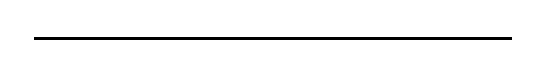
\begin{tikzpicture}
		\draw[thick, black] (0.25*\textwidth, 0) -- (0.75*\textwidth, 0);
		\node[rotate = 360 - 90, xshift = -0.6pt, yshift = 1pt] at (0.25*\textwidth,0){\decotwo};
		\node[rotate = 90, xshift = -0.6pt, yshift = 1pt] at (0.75*\textwidth,0){\decotwo};
	\end{tikzpicture}
	\end{center}
}

\pagestyle{fancy}

\newcommand{\lecday}[1][]
{
    \def\datee{#1}
    \fancyhead[L]{\datee}
}



\newcommand{\signature}
{
	\begin{tikzpicture}[remember picture,overlay]
		\node[fill = YellowOrange!20!white] at ([yshift = 1cm, xshift = -3cm]current page.south east) {\fontsize{10pt}{0pt}{\itshape Kara.$\mathcal{A}$}};
	\end{tikzpicture}
}

\AddToHook{shipout/background}{
  \begin{tikzpicture}[remember picture, overlay]
	  \node[] at ([yshift = 1.5cm,xshift = \textwidth /2 + 0.9cm]current page.south west) {\includegraphics[width = 0.5cm]{preview3}};
	  \node[] at ([yshift = 1.5cm,xshift = - \textwidth /2 - 0.9cm]current page.south east) {\includegraphics[width = 0.5cm]{preview4}};
  \end{tikzpicture}
}



\newtcolorbox[auto counter, number within = section]{remark}[1][]
{
       		title = Remark #1,
		enhanced,
		boxrule = 0pt,
		colback = white,
		breakable,
		arc = 4pt,
		colbacktitle = cyan,
		colback = cyan!5!white,
		segmentation style =
		{
			solid,cyan,thick,
		},
		attach boxed title to top left =
		{
			xshift = 0cm,
		},
		boxed title style =
		{
			boxrule = 0pt,
			sharp corners,
			drop fuzzy shadow = {cyan},
		},
		drop fuzzy shadow = {cyan!80!black},
}

\newtcolorbox[auto counter, number within = section]{theorem}[1][]
{                                      
		title = Theorem \thetcbcounter : #1,
		enhanced, 
		boxrule = 0pt,
		colback = white,
		breakable,
		arc = 4pt,
		colbacktitle = purple,
		colback = purple!5!white,
		segmentation style = 
		{
			solid, purple,thick,
		},
		attach boxed title to top left = 
		{
			xshift = 0cm, 
		},
		boxed title style = 
		{
			boxrule = 0pt,
			sharp corners,
			drop fuzzy shadow = {purple},
		},
		drop fuzzy shadow = {purple!80!black},
}

\newtcolorbox[auto counter, number within = section]{definition}[1][]
{                                      
		title = Definition \thetcbcounter : #1,
		enhanced, 
		boxrule = 0pt,
		colback = white,
		arc = 4pt,
		breakable,
		colbacktitle = YellowOrange!80!black,
		segmentation style = 
		{
			solid, YellowOrange,thick,
		},
		attach boxed title to top left = 
		{
			xshift = 0cm, 
		},
		colback = YellowOrange!5!white,
		boxed title style = 
		{
			boxrule = 0pt,
			sharp corners,
			drop fuzzy shadow = {YellowOrange!80!orange},
		},
		drop fuzzy shadow = {YellowOrange!80!black},
}

\newtcolorbox[auto counter, number within = section]{corollary}[1][]
{                                      
		title = corollary \thetcbcounter : #1,
		enhanced, 
		boxrule = 0pt,
		colback = white,
		arc = 4pt,
		breakable,
		colbacktitle = YellowOrange!80!black,
		segmentation style = 
		{
			solid, YellowOrange,thick,
		},
		attach boxed title to top left = 
		{
			xshift = 0cm, 
		},
		colback = YellowOrange!5!white,
		boxed title style = 
		{
			boxrule = 0pt,
			sharp corners,
			drop fuzzy shadow = {YellowOrange!80!orange},
		},
		drop fuzzy shadow = {YellowOrange!80!black},
}


\newtcolorbox{example}[1][]
{                                      
		title = Example,
		enhanced, 
		boxrule = 0pt,
		colback = white,
		arc = 4pt,
		segmentation style = 
		{
			solid, SpringGreen,thick,
		},
		breakable,
		colback = SpringGreen!5!white,
		colbacktitle = SpringGreen!80!black,
		attach boxed title to top left = 
		{
			xshift = 0cm, 
		},
		boxed title style = 
		{
			boxrule = 0pt,
			sharp corners,
			drop fuzzy shadow = {SpringGreen!80!orange},
		},
		drop fuzzy shadow = {SpringGreen!80!black},
}


\newcommand{\integral}[4]{\int\limits_{#1}^{#2} #4 d#3}
\newcommand{\limit}[3]{\lim\limits_{#1 \rightarrow #2} #3}
\newcommand{\strone}[2]{\left[ \begin{gathered}#1\\ #2\end{gathered} \right] }
\newcommand{\strtwo}[2]{\left\{ \begin{gathered}#1\\ #2\end{gathered} \right\} }
\newcommand{\strthree}[2]{\left\lfloor \begin{gathered}#1\\ #2\end{gathered} \right\rfloor }


\newcommand{\startbf}[1]{\text{\bfseries{#1}}}
\newcommand{\sett}[1]{\left\{ #1 \right\}}
\newcommand{\thesis}[1]{\left( #1 \right)}
\newcommand{\brkt}[1]{\left[ #1 \right]}
\newcommand{\floor}[1]{\left\lfloor #1 \right\rfloor}


\DeclareMathOperator{\img}{im} % Image
\DeclareMathOperator{\Img}{Im} % Image
\DeclareMathOperator{\coker}{coker} % Cokernel
\DeclareMathOperator{\Coker}{Coker} % Cokernel
\DeclareMathOperator{\Ker}{Ker} % Kernel
\DeclareMathOperator{\rank}{rank}
\DeclareMathOperator{\Spec}{Spec} % spectrum
\DeclareMathOperator{\Tr}{Tr} % trace
\DeclareMathOperator{\pr}{pr} % projection
\DeclareMathOperator{\ext}{ext} % extension
\DeclareMathOperator{\pred}{pred} % predecessor
\DeclareMathOperator{\dom}{dom} % domain
\DeclareMathOperator{\ran}{ran} % range
\DeclareMathOperator{\Hom}{Hom} % homomorphism
\DeclareMathOperator{\Mor}{Mor} % morphisms
\DeclareMathOperator{\End}{End} % endomorphism


\newcommand{\lm}{\ensuremath{\lambda}}
\newcommand{\eps}{\ensuremath{\epsilon}}
\newcommand{\veps}{\ensuremath{\varepsilon}}
\newcommand{\al}{\ensuremath{\alpha}}
\newcommand{\bb}{\ensuremath{\beta}}
\newcommand{\cc}{\ensuremath{\gamma}}
\newcommand{\dd}{\ensuremath{\delta}}
\newcommand{\DD}{\ensuremath{\Delta}}
\newcommand{\ff}{\ensuremath{\phi}}
\newcommand{\FF}{\ensuremath{\varphi}}

\newcommand{\RR}{\mathbb{R}}
\newcommand{\RO}{\mathcal{R}}
\newcommand{\EE}{\mathbb{E}}
\newcommand{\CC}{\mathbb{C}}
\newcommand{\RW}{\mathbb{R}^2}
\newcommand{\RT}{\mathbb{R}^3}
\newcommand{\RN}{\mathbb{R}^n}
\newcommand{\DS}{\mathcal{D}}

\newcommand{\KK}{\mathbb{K}}
\newcommand{\KW}{\mathbb{K}^2}
\newcommand{\KT}{\mathbb{K}^3}
\newcommand{\KN}{\mathbb{K}^n}

\newcommand{\NN}{\mathbb{N}}

\newcommand{\PS}{\mathcal{P}}
\newcommand{\AS}{\mathcal{E}}
\newcommand{\FS}{\mathcal{F}}
\newcommand{\LS}{\mathcal{L}}
\newcommand{\MS}{\mathcal{M}}


















\lecday[2025-02-18]

% \begin{document}

\section{Normed Algebra}
\begin{definition}[]

Let $\KK$ be a filed, an algebra over $\KK$ or 
simply a $\KK$-algebra is a $\KK$-vector space a 
$\mathcal{A}$ or $\left( \mathcal{A} ,+,. \right)$  equipped
with a bilinear multiplication operation, 
$ \times   : \mathcal{A}  \times \mathcal{A}   \longrightarrow \mathcal{A}  $
such that 
$\left( A, + , \times   \right)$ is a ring and 
$"\times  "$ is a compatible with scalar multiplication, that 
is 
\[
\forall \lm \in  \KK, 
\forall x,y \in \mathcal{A} : 
\quad 
\left( \lm \cdot x \right) \times y  = 
x \times  \left( \lm \cdot y \right)  = 
\lm \cdot  \left(  x \times y  \right)
\]
\end{definition}
\begin{example}
	For any field $\KK$ and a ny 
	$ n \in \NN $, $\mathcal{M} _{n}\left( \KK \right)$  is 
	$\KK$-algebra
\end{example}
\begin{definition}[]
let $\left( \mathcal{A} , + , \times , \cdot   \right)$ be a 
$\KK$-algebra, an \it algebra-norm \normalfont on $\mathcal{A} $ 
is a norm $\mid \mid \mid  . \mid \mid \mid $ on the 
$\KK$-vector space $\left( \mathcal{A} , + , \cdot  \right)$  
which satisfies in addition the property : 
\[
\mid \mid \mid  y\times x  \mid \mid \mid  
\leq \mid \mid \mid  x \mid \mid \mid  \cdot 
\mid \mid \mid  y \mid \mid \mid 
\]
we say that $\mid \mid \mid   . \mid \mid \mid $  is submultiplicative.
\end{definition}
here are the following axioms of the algebra-norm 
\begin{enumerate}
\item $\mid \mid \mid  x \mid \mid \mid = 0 \implies x = 0_{\mathcal{A} }$  
\item $\mid \mid \mid  \lm x \mid \mid \mid = \left| \lm \right| 
	\cdot \mid \mid \mid  x \mid \mid \mid  \quad 
	\forall  \lm \in \KK, \forall x \in \mathcal{A} $   
\item $\mid \mid \mid  x+y \mid \mid \mid  \leq  \mid \mid \mid  x \mid \mid \mid 
		+ \mid \mid \mid  y \mid \mid \mid \quad 
		\forall  x,y \in \mathcal{A} $  
\item $\mid \mid \mid  x \times y  \mid \mid \mid  \leq 
	\mid \mid \mid  x \mid \mid \mid  \cdot  \mid \mid \mid  y \mid \mid \mid 
	\quad 
	\forall x,y \in  \mathcal{A} $  
\end{enumerate}
\begin{example}
Let $E$ be a N.V.S over $\KK = \RR $ or $\CC $, then 
$\mathcal{L} \left( E,E \right)$ with the laws $+,\cdot ,\circ $  
equipped with the subordinate norm 
$\mid \mid \mid  . \mid \mid \mid $  induced by 
$\| . \| _{E}$ is a normed algebra according to the above proposition
\end{example}
\newpage
\section{An important particular case (matrix norm)}
\begin{definition}[]
Let $n \in \NN$, a matrix norm on $\mathcal{M} _{n} \left( \KK \right)$ 
where $\KK = \RR  \text{ or } \CC $ is a map 
$ \mid \mid \mid  . \mid \mid \mid  : \mathcal{M} _{n}\left( \KK \right) \longrightarrow [0,\infty ) $ 
which satisfies : 
\begin{enumerate}[(i)]
\item $\forall  A \in  \mathcal{M}_{n}\left( \KK \right)  : 
	\quad \mid \mid \mid  A \mid \mid \mid  = 0 
	\implies A = 0_{\mathcal{M} _{n}(\KK) }$ 
\item $\forall  A \in \mathcal{M} _{n}(\KK), 
	\forall \al \in \KK : \quad 
	\mid \mid \mid  \al A \mid \mid \mid = 
	\left| \al \right| \cdot 
	\mid \mid \mid  A \mid \mid \mid $  
\item $\forall A,B \in \mathcal{M} _{n}(\KK) : \quad 
	\mid \mid \mid  A+B \mid \mid \mid 
	\leq  \mid \mid \mid  A \mid \mid \mid + 
	\mid \mid \mid  B \mid \mid \mid $  
\item $\forall  A,B \in \mathcal{M} _{n}(\KK) : 
	\quad \mid \mid \mid  AB \mid \mid \mid \leq 
	\mid \mid \mid  A \mid \mid \mid 
	\cdot \mid \mid \mid  B \mid \mid \mid $  
\end{enumerate}
in other words, a matrix norm is an algebra norm on 
$\left( \mathcal{M} _{n}(\KK) , +, \times , \cdot   \right)$ where
$\times  $  is matrix multiplication and $\cdot $ is scalar multiplication.
\end{definition}
\begin{remark}[]
Let $n \in \NN$, any norm $\| . \| $  on the $\KK$-vector space
$\KK^{n}$ iduces a matrix norm $\mid \mid \mid  . \mid \mid \mid $  on
$\mathcal{M} _{n}(\KK) $, whixh is defined by : 
\[
\mid \mid \mid  A \mid \mid \mid :=
\sup_{x \in \KK^{n} \backslash \left\{ 0_{\KK^{n}}\right\}}  
\frac{\| Ax \| }{\| x \| } = 
\sup_{x \in \KK, \| x \| =1} 
\| Ax \| 
\]
This particular matrix norm is called 
\begin{center}
	"\it The subordinate norm induced by $\| . \| $"  
	\normalfont
\end{center}
\end{remark}
\begin{example}
let $n \in \NN$. 
\begin{itemize}
	\item the subordinate norm on $\mathcal{M}_{n}(\KK)  $ induced
		by the norm of $\| . \| _{1}$  on $\KK^n $  is given by 
		\[
		\| A \| _{1} :=
		\max _{1 \leq j \leq n} 
		\sum_{i=1}^{n} 
		\left| a_{ij} \right| = 
		\sup_{x \in \KK^n  \backslash \left\{ 0_{\KK^n } \right\}}  
		\frac{\| Ax \| }{\| x \| }
		\]
	\item the subordinate matrix norm on $\mathcal{M}_{n}(\KK)  $ induced by
		the norm $\| . \|_{\infty } $  on $\KK^n $ is given by : 
		\[
		\mid \mid \mid  A \mid \mid \mid_{\infty }  := 
		\max_{ 1 \leq i \leq n} \sum_{j=1}^{n} 
		 \left| a_{ij} \right| = 
		 \mid \mid \mid  A^{T} \mid \mid \mid _{1}
		\]
	\item the subordinate norm on $\mathcal{M}_{n}(\KK)  $   
		induced by the norm $\| . \|_{2} $  
		of $\KK^n $ is given by : 
		\[
		\mid \mid \mid  A \mid \mid \mid_{2}  = 
		\sqrt{\rho \left( A^{T}A \right)}  \quad 
		\left( \forall A \in \mathcal{M}_{n}\left( \KK \right)  \right)
		\]
		where $\rho$ denotes the spectral radius of a square matrix $M$
		of $\mathcal{M}_{n}(\KK)  $ 
		\[
		\left( \rho \left( M \right) :=  
			\max \left\{ 
				\left| \lm \right|, \lm
				\in  \sigma _{\CC }   \left( M \right)
			\right\}
		\right)
		\]
		the square root of the eigen values of the positive semi definite
		matrix $A^{T}A$  are called singular values of $A$
		\[
		\mid \mid \mid  A \mid \mid \mid _{2} = 
		\max S.V \left( A \right) \quad 
		\text{ (the largest singular value of $A$) } 
		\]
	\item suppose that $n \geq 2$, we define 
		\[
		\begin{array}{cccc}
			N : &  \mathcal{M} _{n}\left( \KK \right)  & \longrightarrow & [0,\infty ) \\
		
		           &   A& \longmapsto     & N \left( A \right) := 
			   \max _{1 \leq i,j \leq n} \left| a_{ij} \right|\\ 
		\end{array}
		\]
		it's clear that $N$ is a clear norm on $\mathcal{M}_{n} (\KK) $  but it's not
		a matrix norm on it because we have for example 
		\[
			A = 
			\begin{pmatrix}
				1 & 1 & \hdots  &1  \\
				\vdots & \vdots   & \ddots   & \vdots  \\
				 1& 1 & \hdots   & 1  \\
			\end{pmatrix} 
		\]
		we have 
		\[
			A ^2 = 
			\begin{pmatrix}
				1 & 1 & \hdots  &1  \\
				\vdots & \vdots   & \ddots   & \vdots  \\
				 1& 1 & \hdots   & 1  \\
			\end{pmatrix} 
			\times  
			\begin{pmatrix}
				1 & 1 & \hdots  &1  \\
				\vdots & \vdots   & \ddots   & \vdots  \\
				 1& 1 & \hdots   & 1  \\
			\end{pmatrix} 
			= n \times A 
		\]
		so $N \left( A^2  \right) = n$ and $N \left( A \right)^2 = 1 ^2  = 1$  
		then 
		\[
		N (A^2 ) 
		\quad 
		\cancel{ \leq }  \quad 
		 N \left( A \right)^2 
		\]
		thus $N$ is not a matrix norm.
\end{itemize}
\end{example}
\begin{remark}[]
let $n \in \NN$, for any matrix norm $\mid \mid \mid  . \mid \mid \mid $  on 
$\mathcal{M} _{n}(\KK) $, we have $\mid \mid \mid  I_{n} \mid \mid \mid \geq 1$. Indeed, 
\[
\mid \mid \mid  I_{n}^2  \mid \mid \mid  \leq 
\mid \mid \mid  I_{n} \mid \mid \mid ^2 
\]
that is 
\[
\mid \mid \mid  I_{n} \mid \mid \mid  \leq 
\mid \mid \mid  I_{n} \mid \mid \mid ^2 
\]
hence $\mid \mid \mid  I_{n} \mid \mid \mid \geq 1$ 
\end{remark}
\begin{definition}[]
let $n \in \NN$, if a matrix norm $\mid \mid \mid  . \mid \mid \mid $  on 
$\mathcal{M} _{n}(\KK) $ satisfies $\mid \mid \mid  I_{n} \mid \mid \mid  =1$  then it's 
said to be unital
\end{definition}
\begin{example}
	Any suboridnate matrix norm $\mid \mid \mid  . \mid \mid \mid $  
	on $\mathcal{M} _{n}(\KK) $ where $\left( n \in \NN \right)$  induced
	by a norm $\| . \|$ on $\KK^n$ is unital, indeed, in such a case, we have :
	\[
	\mid \mid \mid  I_{n} \mid \mid \mid  = 
	\sup_{x \in \KK^n \backslash  \left\{ 0_{\KK^n } \right\}}  
	\frac{\| I_{n} x \| }{ \| x \| } = 
	\sup_{x \in \KK^n \backslash \left\{ 0_{\KK^n } \right\}}  
	\frac{\| x \| }{\| x \| } = 1
	\]
	note that there exist \it unital matrix norms \normalfont
	on $\mathcal{M}_{n}(\KK)  $  which are not subordinate, (i.e., 
	not induced by any vector space norm $\KK^n $)
\end{example}
\section{The spectral radius of a complex square matrix}
\begin{definition}[]
Let $n \in \NN$ and $A \in \mathcal{M} _{n}(\CC ) $ the spectral radius of $A$, denoted
$\rho (A) $, is the maximum of the modulus of the eigen values of $A$, that is 
\[
\rho (A) :=
\max \left\{ 
	\left|  \lm \right| : \quad 
	\lm \in  \sigma _{\CC }   (A) 
\right\}
\]
we have the following theorem 
\end{definition}
\begin{theorem}[]
let $n \in \NN$ and let $\mid \mid \mid  . \mid \mid \mid $ be a matrix norm on
$\mathcal{M} _{n}(\CC ) $, then for any $A \in \mathcal{M} _{n}(\CC ) $, we have : 
\[
	\rho \left( A \right) \quad  \leq  \quad 
	\mid \mid \mid  A \mid \mid \mid 
\]
\end{theorem}
\begin{proof}
let $A \in \mathcal{M} _{n}(\CC ) $ and let $\lm \in \CC $  be an arbitrary eigen value 
of $A$, so $\exists  x \in \CC ^{n} \backslash  \left\{ 0_{\CC ^n } \right\}$ such that 
$Ax = \lm x$ consider : 
\[
B := \left( X \backslash 0_{\CC ^{n}} \backslash \hdots \backslash 0_{\CC ^n } \right) 
\quad M_{n} \left( \CC  \right) \backslash 
\left\{ 0_{\mathcal{M} _{n}(\CC ) } \right\}
\]
then we have : 
\begin{align*}
	AB &= \left( Ax \mid  A 0_{\CC ^n } \mid  \hdots \mid  A 0_{\CC ^n } \right) \\
          &= 
	  \left( \lm x \mid  0_{\CC ^n } \mid  \hdots \mid  0_{\CC ^n } \right) \\
	  &= 
	  \lm \left( x \mid  0_{\CC n} \mid  \hdots \mid  0_{\CC^n } \right)
	  \\
	  &= \lm B 
\end{align*}
thus 
\[
\mid \mid \mid  AB \mid \mid \mid  = \mid \mid \mid  \lm B \mid \mid \mid  =
\left| \lm \right| \left| B \right|
\]
so 
\[
\lm \mid \mid \mid  B \mid \mid \mid  = 
\mid \mid \mid  A B  \mid \mid \mid  \leq 
\mid \mid \mid  A \mid \mid \mid  \cdot  
\mid \mid \mid  B \mid \mid \mid 
\]
thus 
\[
\left| \lm \right| \leq \mid \mid \mid  A \mid \mid \mid  
\quad \left( \forall  \lm \in  \sigma _{\CC }(A)    \right)
\]
hence
\[
\max _{\lm \in \sigma _{\CC } \left( A \right)  } \left| \lm \right| \leq 
\mid \mid \mid  A \mid \mid \mid    \implies 
\left( \rho (A)  \right) \leq 
\mid \mid \mid  A \mid \mid \mid  
\]
as required 
\end{proof}
\begin{theorem}[Gelfond's formula]
	Let $n \in \NN$  and $\mid \mid \mid  . \mid \mid \mid $  
	be a matrix norm on $\mathcal{M} _{n}(\CC ) $  then for every
	$A \in \mathcal{M} _{n}(\CC ) $, we have
	\[
	\rho(A)  = 
	\lim_{k \to \infty } 
	\mid \mid \mid  A^{k} \mid \mid \mid ^{1/k}
	\]
\end{theorem}
\chapter{Properties of finite-dimensional N.V.S}
\section{Norms on a finite-dimensional \texorpdfstring{$\KK$}{K}-vector space}
Let $n \in \NN$ and $E$ be an $n$-dimensional vector space over $\KK$, 
let also $\mathcal{B} = \left( e_1,e_2, \hdots , e_{n} \right)$ 
be a basis of $E$, using $\mathcal{B} $ we can construct on $E$ several norms including :
\[
\| . \| _{1,\mathcal{B} } \quad 
\| . \| _{2, \mathcal{B} } \quad 
\| . \| _{p, \mathcal{B} } \quad 
\left( p \geq 1 \right) \quad \text{ and }  \quad 
\| . \|  _{\infty ,\mathcal{B} }
\]
defined by 
\begin{align*}
	\| x \| _{1,\mathcal{B} } &:= 
\sum_{i=1}^{n} \left| x_{i} \right| \\
	\| x \| _{2,\mathcal{B} } &:=
\sqrt{\sum_{i=1}^{n} \left| x_{i} \right|^2 }  \\
	\| x \| _{3,\mathcal{B} } &:= 
	\left( 
		\sum_{i=1}^{n} 
		\left| x_{i} \right|^{p}
	\right)^{1/p} \\
	\| x \| _{\infty ,\mathcal{B} } &:= 
	\max _{1 \leq i \leq n} \| x_{i} \| 
\end{align*}
we easily show that these norms on $E$ are all equivalent, lets consider in particular 
the norm $\| . \| _{\infty , \mathcal{B} }$, it's immediate that the map 
\[
\begin{array}{cccc}
        &  \left( \KK^n , \| . \| _{\infty } \right)  & \longrightarrow & \left( 
	       E, \| . \| _{\infty , \mathcal{B} }
       \right) \\

           &   (x_1,x_2, \hdots ,x_{n}) & \longmapsto     &  x_1 e_1 + \hdots + x_{n}e_{n}\\ 
\end{array}
\]
this map is an isometry (bijective), since the distances are conserved 
we call it \it isomorphism isometric \normalfont, it's an homeomorphism
because it's lipschitz, consequently, the $\KK$-N.V.S, 
$\left( E, \| . \| _{\infty , \mathcal{B} } \right)$  and 
$\left( \KK^n  , \| . \| _{\infty }\right)$  have the same toplogical and 
metric properties, in particular, we derive that : 
\begin{enumerate}[(1)]
	\item The N.V.S $\left( E, \| . \|_{\infty , \mathcal{B} }  \right)$  
		is complete (i.e., a Banach space)  
	\item The compact parts of $\left( E, \| . \| _{\infty , \mathcal{B} } \right)$   
		are exactly bounded parts in particular 
		\[
		S_{E} \left( 0_{E},1 \right)|_{ \| . \| _{\infty ,\mathcal{B} }}
	\quad \text{ is compact in } \quad 
	\left( E, \| . \| _{\infty ,\mathcal{B} } \right)
		\]
		these two properties are used to prove the following fundamental
		theorem
\end{enumerate}
\begin{theorem}[]
On a finite-dimensional vector space $\KK = \RR $ or $\CC $, all norms
are equivalent
\end{theorem}
\begin{proof}
	let $n \in \NN$ and $\EE $ an $n$-dimensional vector space over 
	$\KK = \left( \RR  \text{ or } \CC  \right)$, let 
	also $\mathcal{B} = \left( e_1,e_2, \hdots ,e_{n} \right)$  
	be a fixed basis of $E$, we are going to show that every norm on $E$ 
	is equivalent to the norm $\| . \| _{\infty ,\mathcal{B} }$, let $N$ 
	be an arbitrary norm on $E$ and let us show that 
	$N \sim \| . \| _{\infty ,\mathcal{B} }$ on the one hand, 
	by using the properties of $N$ as a norm on $E$, we have for all
	$x = x_1 e_1 + \hdots + x_{n} e_{n}$  with $\left( x_1, \hdots , x_{n} \in \KK \right)$, 
	we have : 
	\begin{align*}
		N \left( x \right) &= 
	N \left( x_1 e_1 + \hdots + x_{n}e_{n} \right) \\ 
				   &\leq 
		N \left( x_1 e_1 \right) + 
		\hdots + N \left( x_{n} e_{n} \right) \\ 
	&= \left| x_1 \right| N \left( e_1 \right) + 
	\left| x_2 \right| N \left( e_2 \right) + \hdots +
	\left| x_{n} \right| N \left( e_{n} \right) \\
	& \leq \left( \max _{1 \leq i \leq n} \left| x_{i} \right|\right) 
	\sum_{i=1}^{n} N \left( e_{i} \right) = 
	\left( \sum_{i=1}^{n} N \left( e_{i} \right) \right) 
	\| x \| _{\infty , \mathcal{B} }
	\end{align*}
	so by setting $\bb  = \sum_{i=1}^{n}N \left( e_{i} \right) > 0$, we have
	\[
	N \left( x \right) \leq 
	\bb  \| x \| _{\infty , \bb } \quad 
	\left( 
	\forall  x \in E
	\right)
	\]
	\end{proof}
% \end{document}
